\documentclass[bibliography=totoc]{scrartcl}
\usepackage[ngerman, english]{babel}
\usepackage{rwukoma}
\usepackage[pdfusetitle]{hyperref}
\usepackage{lipsum,caption}
\usepackage{acronym}
\usepackage{algorithm, algpseudocode}
\usepackage{graphicx}
\usepackage{subcaption}
\usepackage{listings}

\title{Document Scanner}
\author{Leopold Gaube and Florian Betz}
\date{\today}

\begin{document}
	\maketitle
	\tableofcontents

	\clearpage	

    \section{Task Overview}
	Not everybody has a physical document scanner in their own household. 
	However, there are plenty of smartphone apps available that can transform any photograph of a document into a "scanned version" without any distracting background or perspective distortions.
	
	In the following report we will present our own approach for scanning a document in an image.
	We do not want to implement everything from scratch, so we will be using \acs{OpenCV}, an open-source computer vision library that fits our purpose.	
	It is available for C, C++, Python and Java \cite{OpenCV}.
	We will be using Python 3.8. Our code and all test images are available in this \hyperlink{https://gitlab.com/gaubeleo/document-scanner}{Gitlab repository} \cite{Gitlab}.
	
	The algorithm consists of three main parts, each with its own challenges.
	First, we have to localize the document in the image. 
	Then we use a perspective transform from the corner points of the document to the entire span of the image in order to obtain a top-down view without perspective distortions.
	Finally, we use a binary filter to distinguish text from background and save the resulting image as our scanned document.

	We also want our algorithm to work under bad lighting conditions, when the document is rotated at 45° and even when the image was taken from an extreme angle.
	Of course the final image will suffer in quality compared to a document taken under near optimal conditions, but our goal is to still obtain a readable document.
	
	\section{Document Localization}
	Some smartphone scanner apps require the user to mark the four corner points of the document manually, however, we want to automate this process by detecting these points using Computer Vision.
	Detecting the corner points consistently is arguably the hardest and most crucial step of the entire scanner program. 
	
	Our first goal is to find the document outline in the input image, but before that we will do some preprocessing.
	We do not need a high resolution image, so we will reduce the information content by first downsizing the input image to something more manageable.
	We resize the image to 400 pixels on the larger side (width or height) and adjust the smaller side according to the original aspect ratio.
	In the process we will also get rid of noise which could potentially reduce the algorithms performance.
	In addition to downsizing the image, we also use a Gaussian Blur (with a 5x5 kernel) in order to smooth the image even further.

	Now we can use a Canny Edge Detector to find locally sudden changes in brightness or color. 
	The resulting binary image distinguishes between edges (depicted as white) and non-edges (black) for each pixel location in the original image.
	The Canny Edge Detector uses two thresholds. 
	All potential edges above the maxValue-parameter will always become an edge and all potential edges below the lowValue will all be rejected.
	Any value in between both thresholds will only be accepted as an edge if the pixel is adjacent to an already existing edge. \cite{Canny}
	
	We are only concerned that the document outline shows up in our edge image, so we chose an upper threshold of 150 which works consistently even for documents on medium contrast backgrounds. 
	However, we encountered a problem that on some images the document outline was missing a single pixel in the edge image and therefore resulting in an unclosed contour.
	That is why we chose a low value of 50 for the lower threshold that helps to increase the chances of obtaining a closed contour.\\
	
	\begin{figure}[h!]
		\centering
		\begin{subfigure}[b]{0.3\linewidth}
			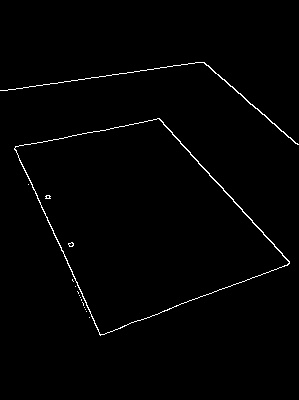
\includegraphics[width=\linewidth]{imgs/edges/extreme_angle.jpg}
		\end{subfigure}
		\hspace{0.2\textwidth}
		\begin{subfigure}[b]{0.3\linewidth}
			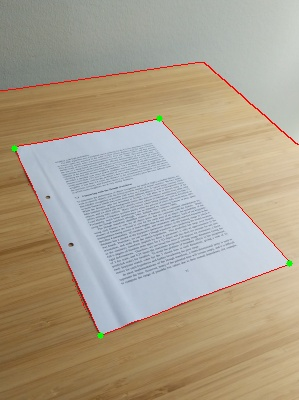
\includegraphics[width=\linewidth]{imgs/contours/extreme_angle.jpg}
		\end{subfigure}
		\caption{The Canny Edge Detector finds edges in all direction (left image). The edge image can in turn be used to detect coherent contours (right image, red lines). The four green dots depict the detected corner points of the document.}
		\label{fig:contours}
	\end{figure}

	From this point on, we have to assume that there exists a closed contour in our edge image which matches the outline of our document. 
	When trying to find the location of the document corners, it is ok if we miss them by a couple of pixels, but detecting the wrong contour would make the resulting document unreadable.

	We use OpenCV's built-in method for finding coherent contours.
	However, we must distinguish the one corresponding to our document from all the other contours in the image.
	Other contours may include text, graphs and pictures on the document itself or even objects e.g. a stapler on the desk. 
	The contour we are looking for should have one of the largest perimeters and it should be able to be approximated it with only four points.
	Both of these assumptions will help us to find the right one, as it is highly improbable that a different contour meets both criteria. 
	We will pick the largest contour that can be approximated using four points as shown by the following code: \\

	\lstset{language=Python}
	\lstset{frame=lines}
	\lstset{label={lst:largest_contour}}
	\lstset{basicstyle=\footnotesize}
	\begin{lstlisting}
# use OpenCV to extract all contours from an edge image
contours, _ = cv.findContours(
	edge_img, mode=cv.RETR_EXTERNAL, method=cv.CHAIN_APPROX_SIMPLE)

largest_contour = None
largest_area = -1
for contour in contours:
	perimeter = cv.arcLength(contour, closed=True)
	
	# approximate the contour using the least amount of vertices 
	# that still satisfy a distance precision of 3%
	low_poly_contour = cv.approxPolyDP(contour, 0.03 * perimeter, closed=True)

	if len(low_poly_contour) == 4:
		# approximate area with a roated rectangle
		((_cx, _cy), (w, h), _angle) = cv.minAreaRect(contour)
		area = w * h
		if area > largest_area:
			largest_area = area
			largest_contour = low_poly_contour
	\end{lstlisting}

	
	\section{Perspective Transformation}
	For the document localization part, we have been working with a low resolution image, making the text unreadable.
	Now we want to create a top-down view of the document with readable text, so we need to project the detected corner points back onto the original resolution. 

	When detecting contours, OpenCV does not care about the order of the points which may result in a rotated image when applying the perspective transformation.
	Therefore, we must first sorts our corner points in a consistent manner.

	OpenCV provides a function for automatically calculating a perspective transformation matrix. 
	It maps our detected (sorted) corner points to the corresponding image corners.
	This matrix can in turn be used to apply this transformation to our input image in order to obtain a top-down view of our document.\\

	\lstset{language=Python}
	\lstset{frame=lines}
	\lstset{label={lst:perspective_transformation}}
	\lstset{basicstyle=\footnotesize}
	\begin{lstlisting}
# sort corners on their relative position [top left, bottom left, top right, bottom right]
sorted_corners = sort_corners(doc_corners)

src = np.array(sorted_corners, dtype="float32")
dst = np.array([[0, 0], [0, HEIGHT], [WIDTH, 0], [WIDTH, HEIGHT]], dtype="float32")

M = cv.getPerspectiveTransform(src, dst)
top_down_img = cv.warpPerspective(img, M, (WIDTH, HEIGHT))
	\end{lstlisting}
    
	\section{Thresholding}
	For the last step of our project we convert the scanned document into a binary image, thus each pixel is supposed to be either black for text and graphs or white for the background.
	The easiest way to achieve this is by converting the color image into grayscale and setting a threshold value. 
	Any pixel value below this threshold would become black, pixel values above would be set to white.

	However, there is a problem with this simple thresholding approach, as it performs poorly under bad lighting conditions as can be seen in [Fig. 3a].
	When taking pictures of documents, a user may cast a shadow with their camera or mobile phone onto the document. 
	This can be problematic if a region in the shadows has lower pixel values for the background than the text in a well-lit region.
	In such a scenario, it would be impossible to find a static threshold that works well for the entire document.
	So instead we need an adaptive approach that looks at a set of neighboring pixels and chooses a threshold for this local region dynamically. \\

	\begin{figure}[h!]
		\centering
		\begin{subfigure}[b]{0.3\linewidth}
			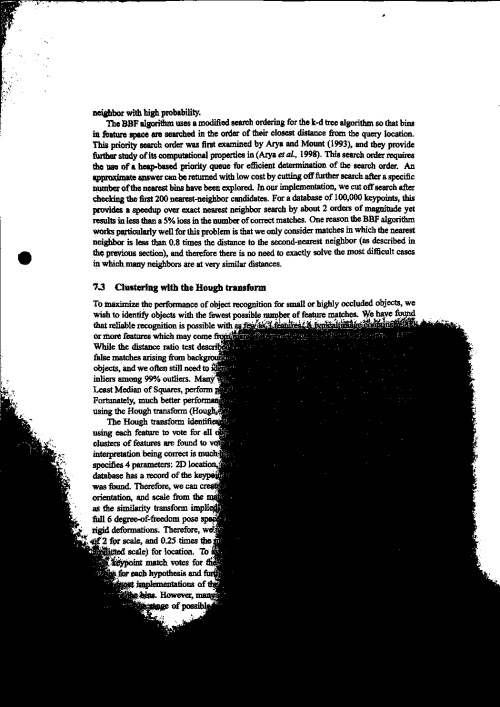
\includegraphics[width=\linewidth]{imgs/threshold/bad_lighting_simple.jpg}
		\end{subfigure}
		\hspace{0.2\textwidth}
		\begin{subfigure}[b]{0.3\linewidth}
			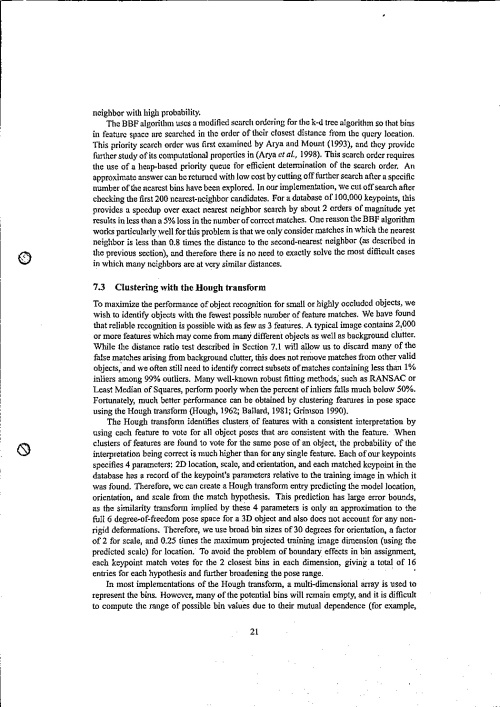
\includegraphics[width=\linewidth]{imgs/threshold/bad_lighting_adaptive.jpg}
		\end{subfigure}
		\caption{A cast shadow may result in unreadable text when using a fixed threshold value (left). Therefore we use an adaptive thresholding method instead (right).}
		\label{fig:thresholding}
	\end{figure}


	The corresponding OpenCV function takes multiple parameters and after some experimenting we settled on a 11 x 11 neighbourhood and a constant C of 5. 
	Furthermore, we prefered the adaptive Gaussian method over the adaptive mean method, making the text look smoother.
	We determined these parameters empirically, depending on which values resulted in the most readable documents.

	It should be noted that an input image with a lot of pixel noise will result in a noisy scanned document.
	In order to reduce the black artifacts we could smooth the image before the thresholding. 
	Unfortunately it would also compromise the text readability and is therefore inadvisable. \\

	\begin{figure}[h!]
		\centering
		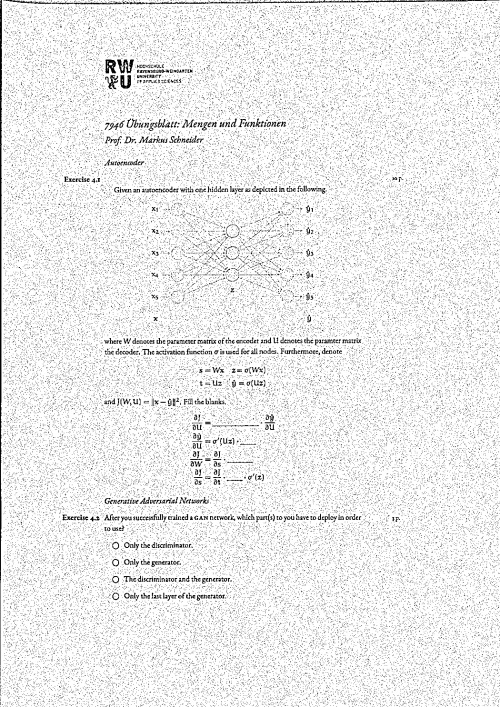
\includegraphics[width=0.3\linewidth]{imgs/threshold/noise.jpg}
		\caption{A high noise images produce small black artefacts in the final scanned document. This is a minor inconviniance, because the text is still readable. This image was taken with a \acs{DSLR} camera using an ISO setting of 3200.}
		\label{fig:noise}
	\end{figure}

	\section{Known problems and possible solutions}
	Overall, our algorithm works consistently even under difficult lighting conditions or when the picture of the document was taken from an unusual angle.
	However, we also observed some use cases where it fails:\\

	\begin{figure}[h!]
		\centering
		\begin{subfigure}[b]{0.3\linewidth}
			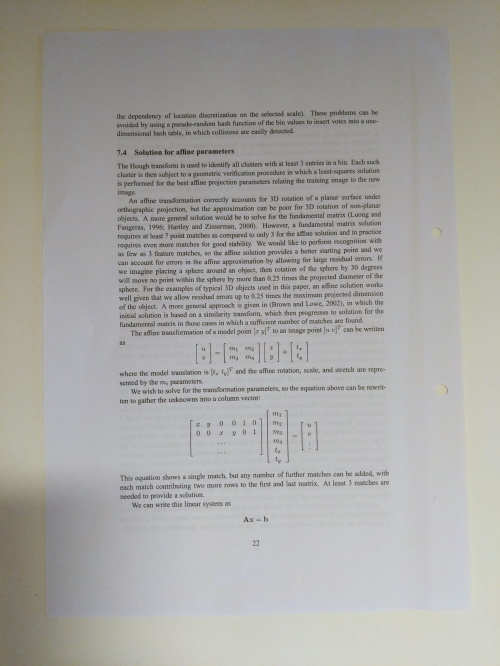
\includegraphics[width=\linewidth]{imgs/not_working/white_background.jpg}
			\caption{A white background results in low contrast around the document outline}
		\end{subfigure}
		\hspace{0.02\textwidth}
		\begin{subfigure}[b]{0.3\linewidth}
			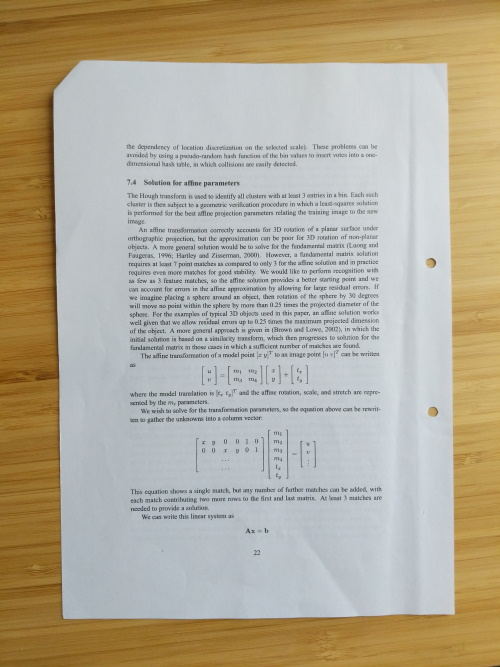
\includegraphics[width=\linewidth]{imgs/not_working/bent_corner.jpg}
			\caption{A document with a bent corner is hard to approximate with a four point contour}
		\end{subfigure}
		\hspace{0.02\textwidth}
		\begin{subfigure}[b]{0.3\linewidth}
			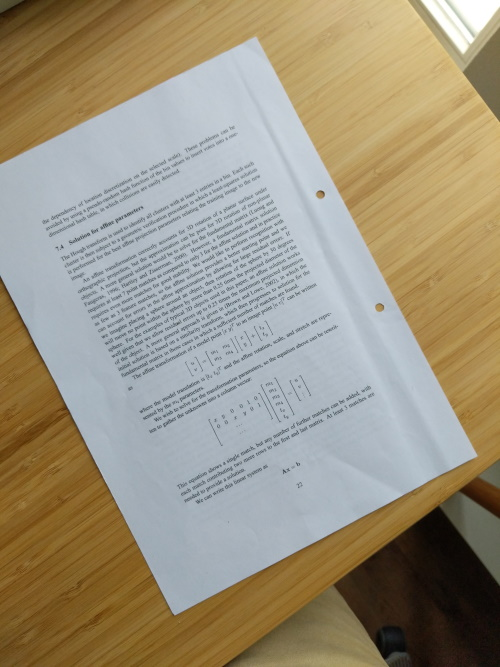
\includegraphics[width=\linewidth]{imgs/not_working/missing_corner.jpg}
			\caption{One of the document corners is cut off from the image composition}
		\end{subfigure}
		\caption{These are example images on which our algorithm (currently) does not work properly on.}
		\label{fig:known_problems}
	  \end{figure}
	
	If the document is placed on a low-contrast background (e.g. a white desk), our algorithm has problems detecting an edge where the document outline should be.
	In some cases it may already help to do more preprocessing e.g. contrast enhancement.
	Currently, our program uses the Canny Edge Detector only once with a fixed lower and upper threshold, because this works fine for the majority of images.
	Whenever the document localization fails, we could try to repeat the process with lower thresholds in order to increase our chance of success. 
	This will introduce more edge artifacts in the edge image, but it might also be enough to detect the document outline.

	Another situation in which our program works poorly is with a bent document corner. 
	This may break the localization algorithm, because the detected contour would - theoretically - have to be approximated using five instead of four corner points.
	In some cases with minor bent corners this still works ok, as we allow for an error of 3\% when approximating the document contour(see Fig. 4a) which may still result in a four point contour approximation. 
	The resulting image will definitely have some small distortion due to the inaccurate localization of the bent corner, but at least the algorithm does not fail entirely.
	The same problem arises if the user is not careful while taking the image and accidentally cutting off a single corner from the picture composition.
	
	For the last two problematic use cases, we already have a possible solution in mind: 
	Whenever the document localization fails, we could try a completely different approach using a Hough Transformation. 
	Hough Transformations are very good at detecting straight lines in edge images. 
	Detecting the four most prevalent lines (with maximum-supression) in an edge image, corresponds to detecting the most likely document edges.
	The intersections of any two lines give us the location of each document corner. 
	A bent/hidden corner or even a corner outside of the image composition should be less of a problem when using the Hough Transformation approach.
	Nevertheless, it has its own downside, because the most prevalent lines have to be document edges and not for instance the edge of a desk.
	Therefore, the Hough Transformation would not replace our approach using contours, but rather act as a backup plan whenever our first document localization fails.\\
	
	\begin{figure}[h!]
		\centering
		\begin{subfigure}[b]{0.3\linewidth}
			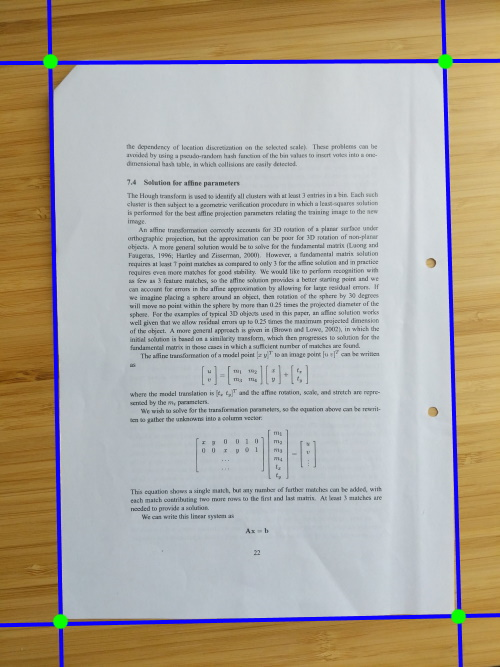
\includegraphics[width=\linewidth]{imgs/not_working/bent_corner_hough.jpg}
		\end{subfigure}
		\hspace{0.1\linewidth}
		\begin{subfigure}[b]{0.4\linewidth}
			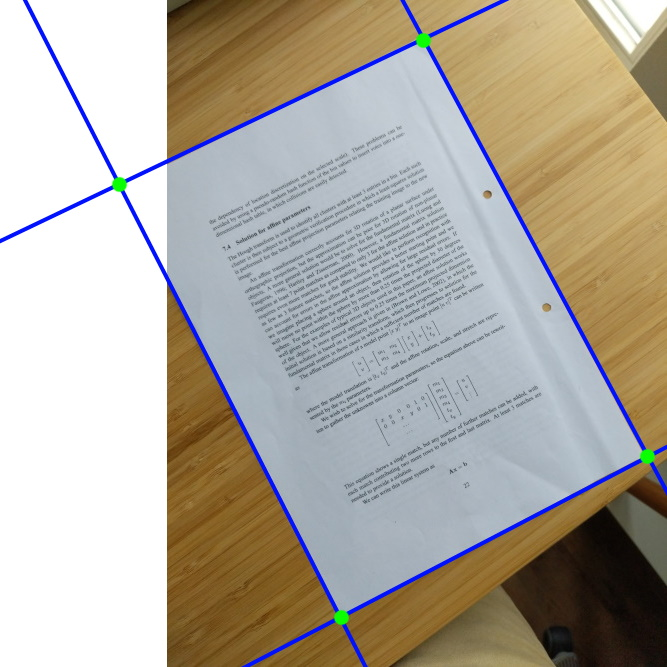
\includegraphics[width=\linewidth]{imgs/not_working/missing_corner_hough.jpg}
		\end{subfigure}
		\caption{A Hough Transformation for detecting the four most prevalent lines (in blue). Using the intersections of these lines could potentially fix problems with missing corners. Both figures were created manually and are for illustrative purposes only.}
		\label{fig:missing_corner_hough}
	\end{figure}

\clearpage
\section*{List of Acronyms} 
\addcontentsline{toc}{section}{List of Acronyms}

\begin{acronym}[....]
    \acro{OpenCV}{Open Source Computer Vision Library}
	\acro{DSLR}{Digital Single Lens Reflex}
\end{acronym}
\bibliographystyle{alpha}			
\bibliography{literature}
\end{document}
